\section{Introduction}

\begin{wrapfigure}[18]{r}{0.45\textwidth}
   \vspace{-40pt}
   \centering
   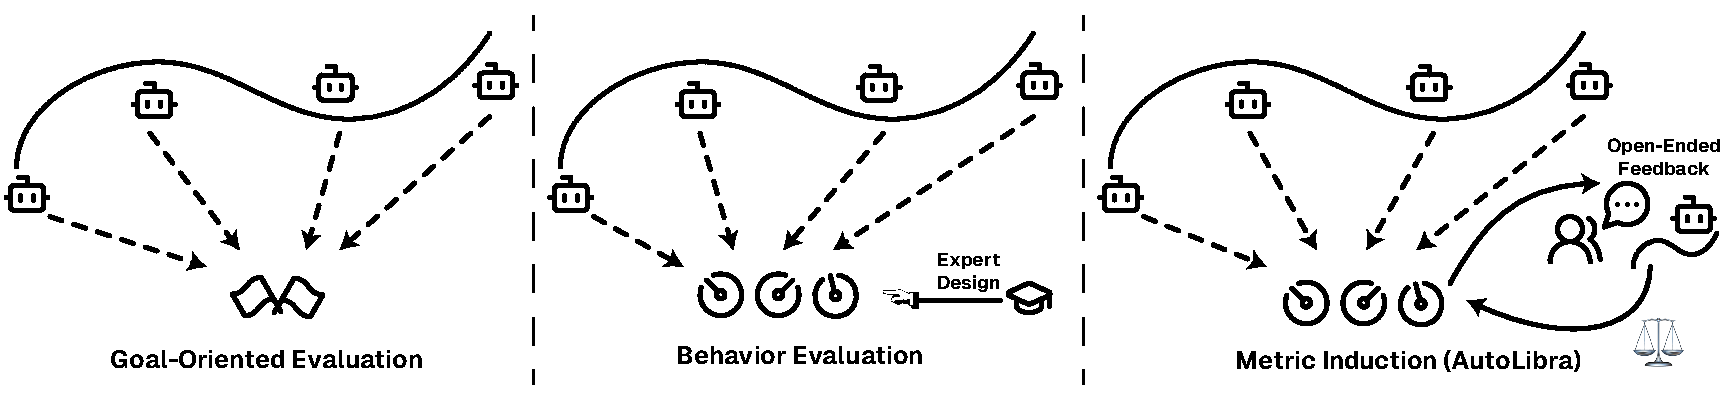
\includegraphics[width=0.45\textwidth]{figs/autolibra.pdf}
   \caption{AutoLibra provides behavioral evaluation on agent performance
    through automatic metric induction based on human feedback and agent trajectories.}
\end{wrapfigure}


Efficient human learners internalize open-ended feedback from others into self-regulation metrics
\citep{pintrich2002development,nicol2006formative}.
These metrics offer lenses for self-reflection on the
strengths and weaknesses of ourselves and ladders for self-improvement.
In this paper, we ask:
\textbf{can we automatically induce metrics to evaluate and improve language agents from natural language feedback?} 

   
The current evaluation of large language model (LLM) agents and reward modeling often fall
into two paradigms: (1) goal-oriented evaluation --
\emph{whether the agents have fulfilled the given task},
\emph{e.g.} benchmarks \citep{zhouwebarena,jimenezswe,chan2024mle,paglieri2024balrog} and reward
modeling approaches \citep{pan2024autonomous,chen2025scaling,choudhury2025process}
and (2) behavior evaluation -- \emph{how well the agents do on heuristically designed dimensions},
\emph{e.g.} social agent and human-agent interaction benchmarks \citep{zhousotopia,shao2024collaborative}
and agent failure mode analysis \citep{pan2025why,zhang2023effects,yang2023behavioral}. 
Goal-oriented evaluation is often designed to be verifiable through considering, but it is not fine-grained
or comprehensive enough to diagnose agents' behavior problems or find the bottlenecks for improvements \citep{yehudai2025survey}.  
While behavior evaluation complements it, it requires manual design of the metrics either based on top-down heuristics
\citep{zhousotopia}, or thematic analysis of the agent's behavior \citep{shao2024collaborative,pan2025why}.
This manual design process is often time-consuming and labor-intensive through expert annotations and classifications. 

In this paper, we introduce AutoLibra \protect\includegraphics[height=1em]{figs/scale.png},
a metric induction method as a new agent evaluation paradigm 
that mitigates the limitations of the current evaluation paradigms.
This method offers behavior evaluation for agents, with the following advantages:
(1) it provides multi-dimensional behavior evaluation that is fine-grained but requires no manual design of metrics,
(2) it could be applied to different kinds of agents and tasks, and 
(3) the metrics are fully explainable and interpretable by humans.

Taking an inspiration from the code-theme steps of thematic analysis often conducted by human experts in social sciences \citep{braun2006using},
we design the Extraction process of AutoLibra as a two step process:
(1) \emph{grounding}: ground every aspect of the human feedback into a slice of the whole agent trajectory,
and (2) \emph{clustering}: cluster the aspects of all trajectories into multiple clusters of similar behaviors
that can be summarized into metrics. For example, in the context of web agents, the grounding step will
``\textsf{If you find that the button is disabled, don't click it again}'' into a slice of the agent trajectory
``\texttt{action: click[1234]} \texttt{obs: no change} \texttt{action: click[1234]}''. Similar slices where 
agents repeated interact with disabled elements could be clustered into a metric \texttt{repeated-interact-disabled}. 

The Evaluation process of AutoLibra is designed to meta-evaluate the LLM-as-a-Judge results
through matching the detected agent traits with human feedback aspects.


we design AutoLibra as a closed-loop system
that has an \emph{Extraction Step} which extracts metrics from human feedback and agent trajectories,
and an \emph{Evaluation Step} which meta-evaluates the LLM-as-a-Judge results
through matching the detected agent traits with human feedback aspects. 
Through these two steps, AutoLibra optimizes not only for metrics that represents humans' views on the
agents' behavior, but also for the metrics that are suitable for the LLM-as-a-Judge to produce human-aligned
evaluation results.

\begin{wrapfigure}{r}{0.7\textwidth}
    \centering
    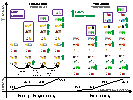
\includegraphics[width=0.7\textwidth]{figs/autolibra-teaser.pdf}
    \caption{Caption}
    \label{fig:enter-label}
\end{wrapfigure}

The Extraction Step of AutoLibra is designed to extract metrics from human feedback and agent trajectories.


With AutoLibra, we aim to answer the following research questions:
\begin{itemize}
    \item \textbf{RQ1:} Can LLMs serve as a proxy for humans when being used in agent behavior thematic analysis,
    behavior evaluation, and meta-evaluating the LLM-as-a-Judge results?
    \item \textbf{RQ2:} What are the differences between the metrics induced by AutoLibra and the behavior evaluation
    metrics designed by human experts?
    \item \textbf{RQ3:} Is AutoLibra useful for improving the performance of agents in different tasks by 
    providing fine-grained behavior evaluation for human agent engineers and agent learning algorithms?
\end{itemize}


